% !TeX program = xelatex
% Local layout based on the official submission-style document.
\documentclass[UTF8,fontset=windows,zihao=5]{ctexart}
\usepackage[a4paper,left=18.01mm,right=20mm,top=20mm,bottom=20mm]{geometry}
\usepackage{amsmath,amssymb,amsthm,bm,booktabs,tabularx,array,graphicx}
\usepackage{setspace,float,caption,xcolor}
\usepackage[numbers,sort&compress,square,super]{natbib}
\usepackage{xurl}
\usepackage[unicode,hidelinks]{hyperref}
\setmainfont{Times New Roman}
\setCJKmainfont{SimSun}[BoldFont=SimHei,ItalicFont=KaiTi]
\setCJKsansfont{SimHei}
\setstretch{1.5}
\setlength{\emergencystretch}{2em}
\setlength{\parindent}{2em}
\setlength{\textfloatsep}{10pt}
\setlength{\intextsep}{10pt}
\setcounter{topnumber}{3}
\renewcommand{\topfraction}{.92}
\renewcommand{\textfraction}{.06}
\renewcommand{\floatpagefraction}{.8}
\captionsetup{font=small,labelsep=quad}
\newcommand{\bicaption}[2]{\caption{#1\\#2}}
\newcommand{\E}{\mathbb E}
\newcommand{\R}{\mathbb R}
\newcommand{\TV}{\operatorname{TV}}
\newcommand{\tr}{\operatorname{tr}}
\newcommand{\Law}{\mathcal L}
\newcommand{\ind}{\mathbf 1}
\newcommand{\norm}[1]{\left\|#1\right\|}
\newtheorem{theorem}{定理}
\newtheorem{lemma}{引理}
\newtheorem{proposition}{命题}
\renewcommand{\proofname}{证明}
\renewcommand{\refname}{参考文献}
\pagestyle{plain}
\ctexset{section={format=\large\heiti},subsection={format=\normalsize\heiti}}
\hypersetup{pdftitle={可信事件记录下的估计损伤界},
 pdfsubject={Finite-horizon estimation damage under trusted event records}}
\begin{document}
\begin{center}
{\heiti\zihao{3}可信事件记录下的估计损伤界\par}
\end{center}
% Author-controlled fields intentionally omitted by the user's instruction.
% Required before uploading: Chinese/English authors and order, affiliations,
% corresponding author and email, funding statement, classification code.
% Do not invent these values or a journal DOI/volume/acceptance date.

\noindent\textbf{摘\quad 要：}
针对事件位和实际预测反馈可信、发送载荷可受有界因果修改的随机触发估计系统，研究统计记录对真实均方误差损伤的约束。利用下一可信事件与协方差标签构造损伤证书，证明在全状态含噪观测、状态矩阵可逆及固定有限时刻下，最坏损伤与攻击幅值平方和记录总变差预算中的较小量同阶。进一步在标量无饱和均匀反馈量化下，证明受限事件与量化遥测记录同律时仍有正损伤，其最坏值具有幅值与精度平方的匹配阶数。数值例证核验损伤分解和格内攻击机制。量化结论不涉及完整接收日志下的隐蔽性。

\smallskip
\noindent\textbf{关键词：}随机事件触发；远程状态估计；统计隐蔽性；可信反馈；量化；估计损伤

\section*{引言}
远程状态估计通过网络利用传感器测量形成系统状态预测。
随机事件触发机制根据量测与预测的偏差决定是否发送，静默事件也参与条件估计。
指数二次触发规则可在适当线性Gaussian模型下保持条件Gaussian结构，为通信与估计分析提供基础\cite{han2015}。
当发送载荷遭到修改时，估计偏差可能经接收端实际预测反馈改变未来发送概率。
可信事件因此可能提供关于隐藏估计损伤的统计信息。

统计隐蔽与估计退化的关系已有广泛研究\cite{bai2017,shang2022,guo2025,song2022,xu2023,wei2026}。
相关成果包括随机事件估计的创新分布、攻击调度、条件矩约束、可信与可疑信息源以及序贯检测。
王彩云等\cite{wang2021}在Kullback--Leibler（KL）散度检测约束下求解最优线性攻击；
陈佳玲等\cite{chen2025}结合水印与参数辨识研究不确定电力系统的攻击检测。
这些工作分别面向攻击优化或检测方法；本文考察既定可信记录对全部允许有界因果策略能提供多强的损伤保证。

表\ref{tab:related}给出直接近邻的定理级对照。CGC指complete Gaussian crater分布\cite{shang2022}。
不同文献的攻击权限和隐蔽准则并不相同，条件矩约束与联合记录总变差（total variation，TV）不能直接互换。
\begin{table}[ht]
\centering\footnotesize
\bicaption{与直接近邻的定理级对照}{Table \thetable\quad Theorem-level comparison with closely related studies}
\label{tab:related}
\begin{tabularx}{\linewidth}{>{\raggedright\arraybackslash}p{1.55cm}*{4}{>{\raggedright\arraybackslash}X}}
\toprule
Study & Trusted information and feedback & Attack permissions & Stealth constraint & Performance result\\
\midrule
Shang et al.\cite{shang2022} &
Local event trigger; attacked remote prediction is not its center &
Manipulation of innovation and communication channels &
CGC distribution and prescribed attack conditions &
Error-covariance recursion (Thm.~2); stealthy constructions (Thm.~3, Cor.~3)\\
Guo et al.\cite{guo2025} &
Local innovation sent each time; events schedule the attack &
Policies under specified information; comparison includes nonlinear feasible policies &
Conditional mean and covariance on attack branches &
Conditional damage optimum for the stated history and schedule (Thm.~1)\\
Wei et al.\cite{wei2026} &
Reliable data and sequential tests; healthy prediction may be broadcast &
Attacks with specified access to reliable and suspicious data &
Gaussian laws, temporal and cross-information moments &
Worst error in the stated feasible set (Thm.~2); necessary and sufficient rank condition for nontrivial attacks without reliable-data access (Cor.~1)\\
Li et al.\cite{li2026} &
Forward innovation quantization; feedback-assisted attack &
Continuous innovation falsified before detection and binary quantization &
Prescribed detector and feasibility constraints &
Sign-probability attack optimization (Thm.~3); covariance convergence (Thm.~4)\\
This study &
Trusted event decisions and faithful actual prediction feedback &
Bounded causal payload changes after genuine transmission &
TV of a specified joint record; zero TV in the quantized extension &
Finite-time worst-case damage orders; residual damage under restricted quantized telemetry\\
\bottomrule
\end{tabularx}
\end{table}

可信信息能够排除某些非平凡隐蔽攻击已有直接先例，特别是Wei等在可靠信息不可读时给出的秩条件\cite{wei2026}。
本文不将这一广义认识作为新发现。Song等允许在发送决定前替换预测反馈；
Xu等和Wei等的分析也允许向传感器广播健康预测\cite{song2022,xu2023,wei2026}。
本文要求反馈忠实于接收端实际预测，事件位不可伪造，且载荷修改发生在发送决定之后。
这种时序使修改引起的偏差保留在下一可信事件的条件概率中。
结合协方差标签对事件历史选择的校准，可进一步得到指定联合记录TV与真实均方误差（mean-square error，MSE）损伤之间的有限时域定量关系。

TV本身不能控制无界平方损失。本文利用有限峰值及上述事件概率关系，
对全部允许的历史相关、量测相关因果策略建立统一上界；
再以合法单拍构造证明最坏损伤在攻击幅值平方与记录TV预算中的较小量上具有匹配阶数。
该结果给出既定协议的充分性能保证及其阶数紧性，不提供一般精确最优攻击或新的检测器。

前向量化观测下的篡改、反馈辅助创新修改及调度防护已有直接成果\cite{li2026,li2025}，
事件触发与量化创新的联合估计也已有研究\cite{shen2025}。
本文的正文扩展只量化参与实际触发的预测反馈中心，保持发送载荷连续。
标量无饱和量化下，内部预测在同一量化格中变化而下一反馈码不变，
可使指定可信事件与量化遥测记录同律时仍存在正损伤；其最坏值具有匹配的幅值--精度阶数。
该结果刻画原保证在特定协议和受限记录下的失效边界，不是所有量化估计系统的普遍安全损失。

受限遥测是一项明确的信息结构假设。远端估计器拥有连续载荷和内部预测，
外部审计者可仅访问指定可信字段；载荷未经认证并不意味着它不可观察。
字段选择接口具有现有规范依据\cite{opcdata}，但本文未验证某工业部署满足全部信任假设，
也未证明这种接口比完整载荷认证成本更低。

\section{系统、信息与损伤模型}
\subsection{精确反馈协议}
考虑固定有限维线性Gaussian模型
\begin{equation}
{\bm{x}}_{t+1}={\bm{A}}{\bm{x}}_t+{\bm{w}}_t,\qquad {\bm{y}}_t={\bm{x}}_t+{\bm{v}}_t .
\label{eq:model}
\end{equation}
设 ${\bm{x}}_0\sim N({\bm{m}}_0,{\bm{P}}_0)$，${\bm{w}}_t\sim N(0,{\bm{Q}})$，${\bm{v}}_t\sim N(0,{\bm{R}})$，
${\bm{P}}_0,{\bm{R}},{\bm{Z}}\succ0$，${\bm{Q}}\succeq0$，${\bm{A}}$可逆；初态、全部过程噪声、量测噪声和触发随机数相互独立。
物理系统不受估计输出控制，不包含自然丢包、时延或乱序。
传感器取得可信实际预测${\bm{m}}_t^-$后，使用私有独立$U_t\sim\mathrm{Unif}[0,1]$决定
\begin{equation}
\gamma_t=0\quad\Longleftrightarrow\quad
U_t\le g({\bm{y}}_t-{\bm{m}}_t^-),\qquad g({\bm{z}})=e^{-{\bm{z}}^\top {\bm{Z}}{\bm{z}}/2}.
\label{eq:trigger}
\end{equation}
发送位已确定后，载荷变为$\tilde {\bm{y}}_t={\bm{y}}_t+{\bm{a}}_t$，
$\norm{{\bm{a}}_t}\le b$；静默时${\bm{a}}_t=0$。

令 ${\bm{R}}_1={\bm{R}},\ {\bm{R}}_0={\bm{R}}+{\bm{Z}}^{-1}$，
${\bm{K}}_i({\bm{P}})={\bm{P}}({\bm{P}}+{\bm{R}}_i)^{-1}$，$F_i({\bm{P}})={\bm{P}}-{\bm{P}}({\bm{P}}+{\bm{R}}_i)^{-1}{\bm{P}}$。
接收器按既定名义规则更新
\begin{align}
{\bm{m}}_t^+&={\bm{m}}_t^-+\gamma_t{\bm{K}}_1({\bm{P}}_t^-)(\tilde {\bm{y}}_t-{\bm{m}}_t^-),&
{\bm{P}}_t^+&=F_{\gamma_t}({\bm{P}}_t^-),\label{eq:receive}\\
{\bm{m}}_{t+1}^-&={\bm{A}}{\bm{m}}_t^+,& {\bm{P}}_{t+1}^-&={\bm{A}}{\bm{P}}_t^+{\bm{A}}^\top+{\bm{Q}}.\nonumber
\end{align}
初值为$({\bm{m}}_0,{\bm{P}}_0)$。${\bm{P}}_t^\pm$是由事件历史确定的名义协方差标签；
在受攻时，它不能单独代表实际接收估计器的真实MSE。

\subsection{信息域与合法策略}
用$\omega_a$表示独立于物理过程和触发随机数的修改方私有种子，
$Y_t^{\rm true}={\bm{y}}_t$在发送时成立，否则为$\bot$。
定义扩充分析信息
\[
\mathcal G_t^-=\sigma(\omega_a,\gamma_{0:t-1},Y^{\rm true}_{0:t-1}),\qquad
\mathcal G_t^+=\mathcal G_t^-\vee\sigma(\gamma_t,Y_t^{\rm true}).
\]
允许任意$\mathcal G_t^+$可测且满足峰值的随机因果策略。
策略不能读取真实状态、未发送量测、未来噪声或$U_t$。
给定策略，已实施动作和接收预测可由上述历史重建。
扩充信息用于证明条件分布，不授予审计者真实量测副本。

固定目标$k$，损伤为同一协议内部的真实MSE增量
\begin{equation}
J_k(\pi)=\E_\pi\norm{{\bm{x}}_k-{\bm{m}}_k^+}^2-\E_0\norm{{\bm{x}}_k-{\bm{m}}_k^+}^2.
\label{eq:damage}
\end{equation}
单个策略的增量可为负；零策略可行，最坏值非负。
令$H_{k+1}$为截至$k+1$的可信事件、实际预测反馈和实际收到的载荷日志。
考虑记录
\[
R_{\rm full}=H_{k+1},\qquad
R_{\rm bits}=\gamma_{0:k+1},\qquad
R_m=({\bm{P}}_k^+,\gamma_{k+1}).
\]
定义
\begin{equation}
\Delta_R(\pi)=\TV(\Law_\pi(R),\Law_0(R)),\qquad
V_R^{(k)}(b,\varepsilon)=
\sup_{\pi:\,\norm{{\bm{a}}_t}\le b,\,\Delta_R(\pi)\le\varepsilon}J_k(\pi).
\label{eq:value}
\end{equation}
本文取$\TV(\mu,\nu)=\sup_B|\mu(B)-\nu(B)|$，向量范数为欧氏范数，矩阵范数为其诱导谱范数。
TV约束为总体分布条件，既非一次运行的观测值，也非预设误报率。
任意仅使用该记录的检验，其攻击与健康拒绝概率之差不超过$\Delta_R$；
这一标准性质解释了统计隐蔽预算的含义。

\subsection{评价者与记录可信性}
远端估计器拥有连续载荷及内部预测，外部审计者可只订阅已规定的可信事件和控制反馈。
载荷未经完整性保护不妨碍保存收到的值；是否向审计者提供它由所规定的信息接口决定。
本文量化扩展把审计者限制为控制遥测订阅者，增强审计则明确加入额外字段。
静默与缺包必须区分，反馈码必须对应传感器实际采用的值，模型版本及初始化已知。
若这些条件不成立，不能直接应用下面的保证。

\section{可信事件记录的损伤保证}
\subsection{真实损伤分解与可观测证书}
给定$\mathcal G_t^\pm$，真实状态仍具有Gaussian条件分布，条件均值记${\bm{\mu}}_t^\pm$，
协方差为${\bm{P}}_t^\pm$。发送并给定真实测量后，事件似然因子在后验归一化时消去；
静默时，积分量测噪声得到以实际预测为中心的Gaussian似然。该结构不要求载荷修改与当前量测独立。
令${\bm{d}}_t={\bm{\mu}}_t^--{\bm{m}}_t^-$、${\bm{D}}_t={\bm{\mu}}_t^+-{\bm{m}}_t^+$，则
\begin{align}
{\bm{D}}_t&=({\bm{I}}-{\bm{K}}_{\gamma_t}({\bm{P}}_t^-)){\bm{d}}_t-\gamma_t{\bm{K}}_1({\bm{P}}_t^-){\bm{a}}_t,\qquad
{\bm{d}}_{t+1}={\bm{A}}{\bm{D}}_t,\label{eq:bias}\\
J_k&=\E_\pi\norm{{\bm{D}}_k}^2+
\E_\pi\tr {\bm{P}}_k^+-\E_0\tr {\bm{P}}_k^+.\label{eq:split}
\end{align}
式\eqref{eq:split}由条件零均值残差的正交性得到。最后两项不能删除；
事件概率改变可能使其为负。

固定${\bm{P}}={\bm{P}}_k^+$，记下一静默位$Y=\ind_{\{\gamma_{k+1}=0\}}$，定义
\begin{align}
{\bm{\Sigma}}({\bm{P}})&={\bm{A}}{\bm{P}}{\bm{A}}^\top+{\bm{Q}}+{\bm{R}},\qquad
s({\bm{P}})=\det({\bm{I}}+{\bm{Z}}^{1/2}{\bm{\Sigma}}({\bm{P}}){\bm{Z}}^{1/2})^{-1/2},\nonumber\\
{\bm{H}}({\bm{P}})&=\tfrac12 {\bm{A}}^\top[{\bm{Z}}^{-1}+{\bm{\Sigma}}({\bm{P}})]^{-1}{\bm{A}},\qquad
W=Y/s({\bm{P}}).
\end{align}
真实条件创新的均值为${\bm{A}}{\bm{D}}_k$。Gaussian积分给
\begin{equation}
\E_\pi[Y\mid\mathcal G_k^+]=s({\bm{P}})e^{-{\bm{D}}_k^\top {\bm{H}}({\bm{P}}){\bm{D}}_k},
\qquad \E_0W=1,\quad \E_\pi W=\E_\pi e^{-{\bm{D}}_k^\top {\bm{H}}({\bm{P}}){\bm{D}}_k}.
\label{eq:witness}
\end{equation}
未来载荷修改发生在未来事件之后，故不改变这一关系。

有限$k$下，P及增益取有限值。由式\eqref{eq:bias}可得
$\norm{{\bm{D}}_k}\le r_kb$。固定$b_{\rm ref}>0$，取
\[
h_*=\min_{\bm{P}}\lambda_{\min}({\bm{H}}({\bm{P}}))>0,\quad
B_*=r_kb_{\rm ref},\quad q=\frac{1-e^{-h_*B_*^2}}{B_*^2}>0.
\]
其中${\bm{A}}$可逆保证$h_*>0$。割线不等式给出
\begin{proposition}[可信下一事件的总体损伤证书]
对全部允许策略及$0\le b\le b_{\rm ref}$，
\begin{equation}
J_k\le \frac{1-\E_\pi W}{q}
+\E_\pi\tr {\bm{P}}_k^+-\E_0\tr {\bm{P}}_k^+.
\label{eq:certificate}
\end{equation}
\end{proposition}
\begin{proof}
在$\norm{{\bm{D}}_k}\le B_*$上，
$1-e^{-{\bm{D}}_k^\top {\bm{H}}({\bm{P}}){\bm{D}}_k}\ge q\norm{{\bm{D}}_k}^2$。
对式\eqref{eq:witness}取期望并代入式\eqref{eq:split}即得。
\end{proof}
右侧是由可信事件与已知模型标签定义的总体统计量，不需要审计者知道攻击向量或真实状态。
有限样本估计仍有统计余量；一个事件或一条轨迹不能直接认证总体损伤。

\subsection{双预算阶数及完整日志下界}
记$\Delta_m=\Delta_{R_m}$，
令$M=\max_{\bm{P}}1/s({\bm{P}})$，$\Omega_k=\max_{\bm{P}}\tr {\bm{P}}-\min_{\bm{P}}\tr {\bm{P}}$。
因$0\le W\le M$且${\bm{P}}$在记录中，标准TV期望界给
\[
J_k\le(M/q+\Omega_k)\Delta_m.
\]
另一方面，式\eqref{eq:bias}控制偏差平方；每个历史下静默概率相对健康变化为$O(b^2)$。
对有限事件前缀耦合并控制P标签的期望差，得到$J_k\le C_{\rm peak}b^2$。
该第二步不可仅从偏差半径推出而忽略协方差项。

\begin{theorem}[精确反馈的有限时域损伤阶数]
\label{thm:exact}
固定模型、有限维数、目标$k$及$b_{\rm ref}$，存在正有限常数$c,C$，
对$0<b\le b_{\rm ref}$、$0\le\varepsilon\le1$及
$R\in\{R_{\rm full},R_{\rm bits},R_m\}$，
\begin{equation}
c\min\{b^2,\varepsilon\}\le V_R^{(k)}(b,\varepsilon)
\le C\min\{b^2,\varepsilon\}.
\label{eq:exact-bound}
\end{equation}
特别地，$V_R^{(k)}(b,0)=0$。
\end{theorem}
\begin{proof}
上界为两种界的组合及记录的数据处理。
下界在目标前不修改，仅在目标真实发送后使用独立等概率符号$\sigma$和固定单位方向${\bm{v}}$，$\norm {\bm{v}}=1$，
取${\bm{a}}_k=\sigma\eta {\bm{v}}$，其他时刻为零。目标损伤为$L_{\bm{v}}\eta^2$，$L_{\bm{v}}>0$。
给定健康前史，将当前连续载荷和下一静默原子/连续载荷写成一个联合核。
该核对位移二阶连续$L^1$可微，正负混合的一阶项消去，完整日志TV不超过$C_1\eta^2$。
取$\eta=\min\{b,\sqrt{\varepsilon/C_1}\}$完成下界，联合核细节见附录\ref{app:single}。
\end{proof}
单拍构造足够支持阶数，并不声称是精确最坏策略。
常数依赖模型、$k$、$b_{\rm ref}$；$\varepsilon$与$b^2$的量纲通过模型相关常数联系，
两预算切换点不是普遍的$\varepsilon=b^2$。

\subsection{观察时域与信息限制}
式\eqref{eq:witness}使用下一拍可信事件以及目标协方差标签。
因此，定理\ref{thm:exact}不直接适用于只观察到目标拍的日志，或删去历史校准标签后的单个事件边缘。
这一充分保证不声称已确定所有审计方式的最小记录。
精确协方差标签由事件历史决定，但并不天然构成低比特压缩；
本文未给出其固定字长编码或通信成本最优性。

\section{反馈精度与审计信息限制}
\subsection{量化协议及一致静默更新}
本节限于\textbf{标量}系统，$A\ne0$，$P_0,R,Z>0$，$Q\ge0$，并固定有限目标$k$。
量化的是实际预测反馈，前向发送载荷保持连续。取无限格点、无饱和的均匀量化器
\[
c_t=Q_\delta(m_t^-),\qquad Q_\delta(m)=2\delta\left\lfloor\frac{m+\delta}{2\delta}\right\rfloor,
\qquad |c_t-m_t^-|\le\delta,
\]
量化格为半开区间$[2j\delta-\delta,2j\delta+\delta)$，$j\in\mathbb Z$，故并列点归属固定。
传感器用$y_t-c_t$生成原指数二次随机事件。
发送支路保持原更新；静默时必须使用
\begin{equation}
m_t^+=m_t^-+K_0(P_t^-)(c_t-m_t^-),\qquad P_t^+=F_0(P_t^-).
\label{eq:silentq}
\end{equation}
健康条件均值于是与接收均值一致。若仍使用旧的$m_t^+=m_t^-$，
健康运行也会因非零舍入误差产生条件均值失配。

给定扩充真实历史，$c_t$为已知量；静默似然是以$c_t$为中心、噪声$R+Z^{-1}$的Gaussian因子。
发送并给定真实测量后事件因子仍可消去。因此精确条件Gaussian结构保留，
且真实条件均值与接收均值的偏差仍满足式\eqref{eq:bias}。
量化误差项在两者使用同一静默中心后相消。
这个结论不应移到只包含量化码或污染载荷的较小条件信息域。

定义同量化协议内部损伤
\[
J_{k,\delta}=\E_{\pi,\delta}(x_k-m_k^+)^2-\E_{0,\delta}(x_k-m_k^+)^2.
\]
它不含正常量化运行相对正常精确运行的损失。
令$T_{\delta,k}=(\gamma_{0:k+1},c_{0:k+1},P_k^+)$为全部可信控制遥测，
$R_{m,\delta}=(P_k^+,c_{k+1},\gamma_{k+1})$为其投影。
两者都排除连续接收载荷和未量化内部预测。
相应TV与最坏值采用式\eqref{eq:value}的同协议定义。

\subsection{零记录差异下的残余损伤}
令$e=c_{k+1}-m_{k+1}^-$，$P=P_k^+$，
$\Sigma(P)=A^2P+Q+R$，$V(P)=Z^{-1}+\Sigma(P)$，$h(P)=A^2/[2V(P)]$。
下一事件关系变为
\begin{equation}
\E_{\pi,\delta}[W\mid\mathcal G_k^+]
=\exp[-h(P)(D_k-e/A)^2],\qquad W=Y/s(P).
\label{eq:qprob}
\end{equation}
健康时$D_k=0$，所以$\E_{0,\delta}W$一般小于1；
原精确协议的健康归一化不能直接沿用。

\begin{theorem}[标量有限精度的零TV损伤地板]
\label{thm:quant}
固定标量模型、有限$k$、$b_{\rm ref}>0$、$\delta_{\rm ref}>0$。
存在$\delta_*>0$及正有限$c_k,C_k$，使全部
$0<b\le b_{\rm ref}$、$0<\delta\le\min\{\delta_*,\delta_{\rm ref}\}$满足
\begin{equation}
c_k\min\{b^2,\delta^2\}\le V_{R,\delta}^{(k)}(b,0)
\le C_k\min\{b^2,\delta^2\},
\label{eq:quant-bound}
\end{equation}
其中$R=T_{\delta,k}$或$R_{m,\delta}$。
\end{theorem}
\begin{proof}
上界适用于包括目标前动作在内的全部允许策略。
有限前缀集给$|D_k|\le r_kb$。取
$R_*=r_kb_{\rm ref}+\delta_{\rm ref}/|A|$，
$h_*=\min_Ph(P)>0$，
$q_*=(1-e^{-h_*R_*^2})/R_*^2$，
$c_0=\max_P1/[2V(P)]$。
当记录同律，$\E_\pi W=\E_0W$且P标签同律。
由式\eqref{eq:qprob}和健康量化误差界，
\[
q_*\E_\pi(D_k-e/A)^2\le1-\E_\pi W
=1-\E_0W\le c_0\delta^2.
\]
于是
\[
J_{k,\delta}=\E_\pi D_k^2
\le\left(\sqrt{c_0/q_*}+|A|^{-1}\right)^2\delta^2,
\qquad J_{k,\delta}\le r_k^2b^2 .
\]

下界选择此前无动作的合法子类。给定健康真实前史$\zeta$，
令$m=m_k^-$、$e_k=c_k-m$、$P_h=P_k^-$、$S_h=P_h+R$、$K_h=P_h/S_h$。
当前创新$u=y_k-m$的发送次密度为
\begin{equation}
f_{h,e_k}(u)=\phi_{S_h}(u)[1-\exp(-Z(u-e_k)^2/2)].
\label{eq:sentq}
\end{equation}
真实发送后，下一健康预测$M=A(m+K_hu)$可由合法信息计算。
定义开中央半区
\[
\mathcal C_\delta=\bigcup_{j\in\mathbb Z}
(2j\delta-\delta/2,\,2j\delta+\delta/2).
\]
只在真实发送且$M\in\mathcal C_\delta$时，选择独立符号动作$\sigma\eta$，
$\eta=\min\{b,\delta/(2\alpha_{\max})\}$，
$\alpha_{\max}=\max_h|AK_h|$。
因$|AK_h|\eta\le\delta/2$且中央区为开集，两种符号均严格不跨格，下一实际反馈码及事件逐路径相同，
目标前的全部事件/反馈也相同。
独立符号消去目标误差交叉项，故
\[
J_{k,\delta}=\eta^2\E_{0,\delta}[K_h^2\ind_E].
\]
附录\ref{app:uniform}证明安全发送事件的概率在所有健康前史下至少$p_*/4>0$，
从而给出式\eqref{eq:quant-bound}的正下界。
\end{proof}

定理\ref{thm:quant}的常数可依赖$k$，不是长时间一致界。
其下界取目标前无动作策略，只是全允许策略类的合法子集；
不需要也没有假设所有允许攻击此前均无动作。
$\delta^2$在该记录下是不能统一缩为$o(\delta^2)$的余量，
不表示每条运行均有损伤。

\subsection{协议变化与信息变化的区别}
\begin{table}[ht]\centering\small
\bicaption{反馈协议与审计记录的区别}{Table \thetable\quad Feedback protocols and audit records}
\begin{tabularx}{\linewidth}{lXX}
\toprule
Setting & Actual trigger center & Proven guarantee\\
\midrule
A: exact feedback & $m_t^-$ & Zero record TV implies zero worst-case damage.\\
B: quantized feedback & $Q_\delta(m_t^-)$ & Identical telemetry laws allow the residual damage in \eqref{eq:quant-bound}.\\
C: enhanced audit & Same as B & Additional payload or exact prediction information cannot increase worst-case damage; a general zero-damage guarantee is unknown.\\
\bottomrule
\end{tabularx}
\end{table}
仅把A的日志显示值量化，同时传感器仍使用精确中心，不会破坏原先由P和下一事件给出的保证。
B的地板来自量化中心进入实际触发，以及审计者不保留足以区分该见证的连续数据共同作用。

对于定理下界中的独立符号见证，加入目标拍收到的连续载荷后，
统计量$\gamma_k\tilde y_k^2$的期望差为$\eta^2\Pr(E)>0$；
加入下一未量化预测后，其平方期望差为$A^2\eta^2\E[K_h^2\ind_E]>0$。
有限二阶矩下，这些差异证明该见证不再同律。
但排除这个见证不等于排除全部零TV策略；对C只可一般地使用记录投影给出$V_C\le V_B$。

无饱和均匀格代表绝对精度假设，其整数索引没有全路径固定字长。
本文不据此给固定比特部署或认证成本优势，也不将采样估计TV替代上述严格同律证明。

\section{数值例证}
\subsection{精确反馈的二维算例}
本节以两个二维模型和一组预先规定的标量实验核验理论机制。
二维模型为
\[
{\bm{A}}_{\rm S}=\begin{bmatrix}.82&.18\\-.10&.72\end{bmatrix},\qquad
{\bm{A}}_{\rm U}=\begin{bmatrix}1.04&.12\\.03&.91\end{bmatrix},
\]
\[
{\bm{P}}_0=\begin{bmatrix}.8&.12\\.12&.6\end{bmatrix},\quad
{\bm{Q}}=\begin{bmatrix}.05&.01\\.01&.04\end{bmatrix},\quad
{\bm{R}}=\begin{bmatrix}.2&.03\\.03&.3\end{bmatrix},\quad
{\bm{Z}}=\begin{bmatrix}2&.25\\.25&1.5\end{bmatrix}.
\]
目标$k=4$、$b=0.1$。计算考察持续定向策略，以及目标拍随机符号、下一拍补偿的两拍策略。
定理下界采用单拍构造；此处两拍策略作为另一条合法数值见证报告，
不将其数值常数用于单拍证明。

\begin{table}[ht]
\centering\footnotesize
\bicaption{真实目标损伤分解（精确反馈）}{Table \thetable\quad Decomposition of target damage under exact feedback}
\begin{tabular}{llrrr}
\toprule
Model & Policy & Bias energy & Covariance change & Damage $J$\\
\midrule
S & Persistent direction & .001315759 & -.000020445 & .001295314\\
U & Persistent direction & .003252364 & -.000120021 & .003132343\\
S & Two-step sign compensation & .000321850 & 0 & .000321850\\
U & Two-step sign compensation & .000573797 & 0 & .000573797\\
\bottomrule
\end{tabular}
\end{table}
持续策略的协方差变化为负，说明只报告条件偏差平方会高估这些例子的真实损伤。
原两拍策略在目标之前无动作，目标协方差分布不变，所以该项为零。
各组合使用事件树计算；另在$b=0.2$下，对两个模型和两种策略分别以40万次独立重置结果交叉检查。

\begin{table}[ht]
\centering\footnotesize
\bicaption{两拍符号补偿策略的损伤及不同保证（$b=0.1$）}{Table \thetable\quad Damage and distinct guarantees for the two-step sign-compensation policy}
\begin{tabular}{lrr}
\toprule
Quantity & S & U\\
\midrule
True damage & .000321850 & .000573797\\
Population certificate & .000457526 & .000902386\\
Certificate / damage & 1.42155 & 1.57266\\
Upper / witness lower bound (TV-linear region) & 783.639 & 359.136\\
$N=10^4$: mean-centered confidence bound, known reference & .084711 & .072733\\
\bottomrule
\end{tabular}
\end{table}
最后一行按Hoeffding不等式计算，并将经验均值置于总体均值，
不是新采样所得认证结果。总体证书在这两个例子中较接近真实损伤，
有限样本余量却仍很大。双预算曲线只是全策略上界与一条合法构造下界，
不代表真实最优值已经被数值求解。原事件串TV也不替代完整连续日志TV；
后者预算可行性由解析联合核界提供。

\subsection{预先规定的标量验证}
量化扩展仅在标量范围验证。S1/U1取$A=0.82/1.04$，
$m_0=0$、$P_0=0.8$、$Q=0.05$、$R=0.2$、$Z=2$，目标$k=4$，$b=b_{\rm ref}=0.1$。
这些是由旧参数首坐标系数构成的独立标量模型，删除耦合后不等于原二维系统的边缘。
每模型使用预先固定的2048条独立基础物理与触发样本，
在三个精度、A/B协议及健康/正/负分支之间共享样本。
两符号分支取平均以评价等概率符号策略，统计独立单位仍是基础样本。
总共4096个模型内独立样本，73728条短方法分支，各运行至$k+1$事件；
C和A-rounded-log只是现有轨迹的观察字段，没有额外状态递推。

量化精度由固定协方差常数选定：
\[
\delta_{\rm cap}=\min\{0.1,\delta_*/2,\alpha_{\max}b/2\},\qquad
\delta_j=\delta_{\rm cap}\{1/4,1/2,1\},\quad
\eta_j=\delta_j/(2\alpha_{\max}).
\]
参数选择先于随机输入产生，精度列表见表\ref{tab:e1-damage}。
A的$\delta$仅为共同门控和剂量标签，不改变精确触发中心；
B采用实际量化反馈和一致静默更新。
二者分别用自己的合法历史决定目标拍中央格门控，不能调用另一协议的健康反事实。
所有动作在真实发送之后发生，其他时刻无动作。
这里比较的是同形式合法见证，不要求A/B的实际动作概率、能量或通信率完全相等。

独立重算核对了事件时序、健康条件均值、量化码及损伤恒等式。
配对损伤与$K_h^2\eta^2\ind_E$的最大绝对差为$3.66\times10^{-16}$。
以下95\%区间来自1000次按基础样本的配对bootstrap，是见证损伤的探索性区间，不是全策略安全置信界。

\begin{table}[ht]
\centering\footnotesize
\bicaption{B协议的见证损伤：精度主导区域}{Table \thetable\quad Feasible witness damage under B in the precision-dominated regime}
\label{tab:e1-damage}
\begin{tabular}{lrrrr}
\toprule
Model / level & $\delta$ & $10^6\hat J$ & Exploratory 95\% interval ($\times10^6$) & $\hat J/\delta^2$\\
\midrule
S1/1 & .00290706 & .295503 & [.256237,.334963] & .034967\\
S1/2 & .00581412 & 1.239223 & [1.086202,1.391006] & .036659\\
S1/3 & .01162823 & 4.814492 & [4.227691,5.429128] & .035606\\
U1/1 & .00556494 & .785686 & [.703663,.878413] & .025370\\
U1/2 & .01112988 & 2.793531 & [2.458229,3.128096] & .022551\\
U1/3 & .02225976 & 11.211802 & [9.942383,12.533812] & .022627\\
\bottomrule
\end{tabular}
\end{table}
各点均为所构造攻击见证的可达到损伤，而非最坏值$V$的数值求解。
本设计令$\eta$随$\delta$变化且均远小于$b$，只考察精度主导区；
不能据三个点声称数值验证了$\min\{b^2,\delta^2\}$的两个区域或估计出一般渐近指数。
A同剂量的见证损伤在S1中为$2.92\times10^{-7}$至$4.81\times10^{-6}$，
在U1中为$7.76\times10^{-7}$至$1.08\times10^{-5}$，详图\ref{fig:e1}。

\begin{figure}[ht]
\centering
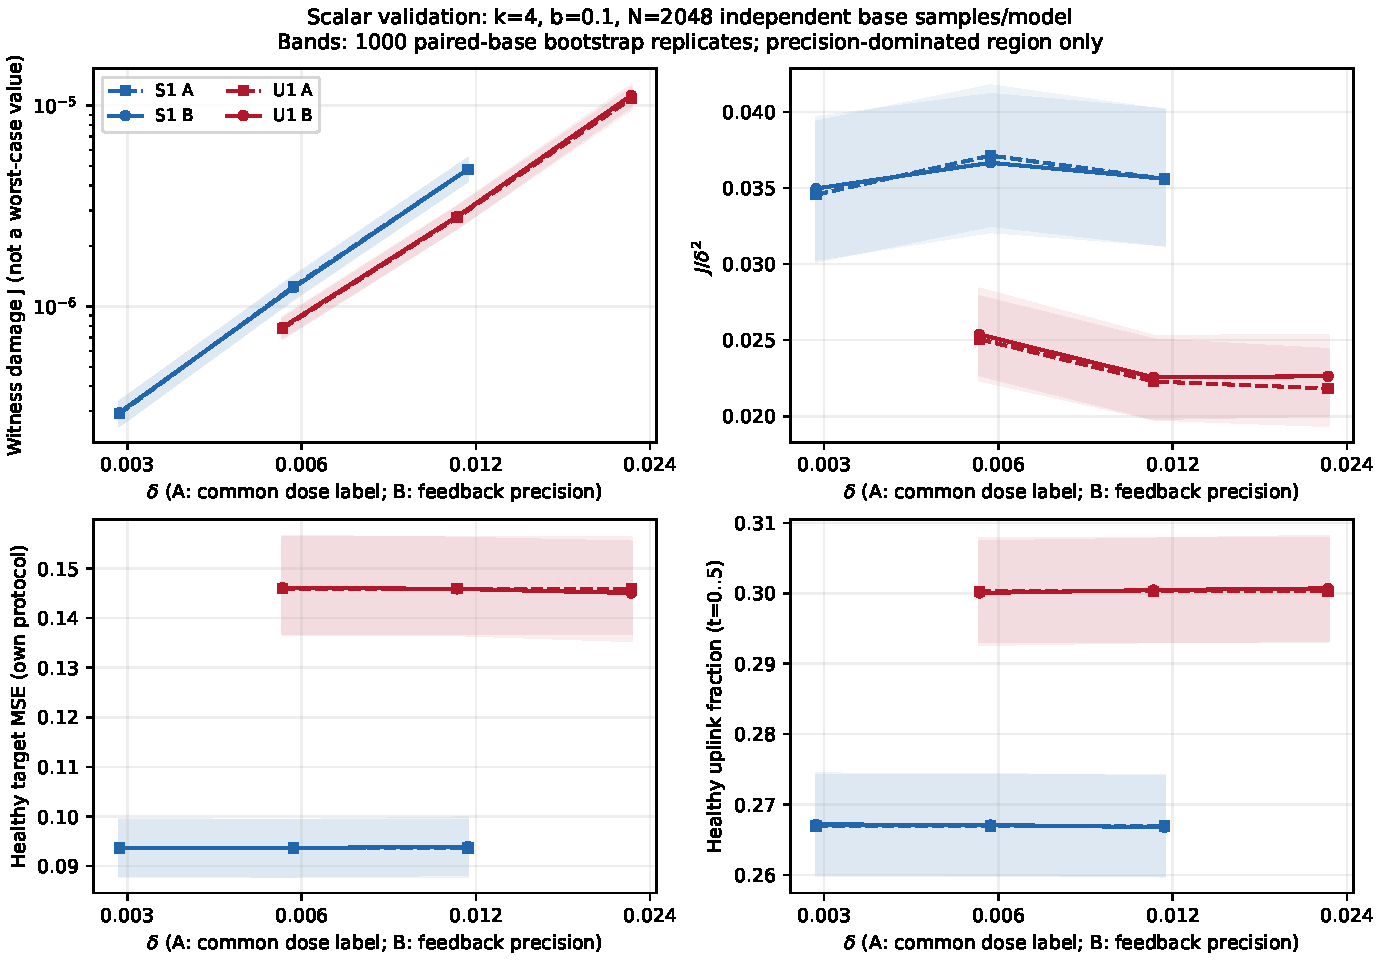
\includegraphics[width=\linewidth]{figures/e1_mechanism.pdf}
\bicaption{标量见证损伤、精度尺度及健康代价；阴影为基础样本配对bootstrap区间}
{Fig. \thefigure\quad Scalar witness damage, precision scaling, and healthy cost.
Shading denotes paired bootstrap intervals. For A, $\delta$ is a dose label; for B, it is the actual feedback precision.}
\label{fig:e1}
\end{figure}

\subsection{各自健康基线及可信记录的一致性}
A的健康MSE在S1/U1分别为0.093640886、0.145956498，
0--5拍平均上行发送率分别为0.266927、0.300293，且不依测试剂量改变。
B各精度结果见表\ref{tab:e1-health}。受攻MSE从相应B健康基线增加，
未把量化本身的健康差异计入攻击损伤。
健康B减A的MSE探索区间在六组中均跨零，点估计有正有负，
不足以主张正常精度或通信收益。
在最大预设精度下，见证损伤约为对应B健康MSE的$0.0051\%$（S1）和$0.0077\%$（U1）。
该量级说明这里验证的是严格正损伤及其精度尺度，不支持“量化导致显著工程损害”的表述。

\begin{table}[ht]
\centering\footnotesize
\bicaption{B的健康和受攻MSE、通信及动作频次}{Table \thetable\quad Healthy and attacked MSE, transmission rate, and attack counts under B}
\label{tab:e1-health}
\begin{tabular}{lrrrr}
\toprule
Model / level & Healthy MSE & Attacked MSE & Healthy Tx rate & Attacks / 2048\\
\midrule
S1/1 & .093701541 & .093701837 & .267171 & 223\\
S1/2 & .093635897 & .093637136 & .267090 & 232\\
S1/3 & .093878253 & .093883067 & .266764 & 225\\
U1/1 & .146129290 & .146130075 & .300049 & 282\\
U1/2 & .145905461 & .145908255 & .300456 & 252\\
U1/3 & .145071599 & .145082811 & .300700 & 252\\
\bottomrule
\end{tabular}
\end{table}
B的健康与两符号运行在所有预定样本中均具有完全相同的事件、量化码和目标P，
与理论逐路径不变性一致；这一抽样检查不代替总体同律的证明。
实际幅值S1依次为0.00442673、0.00885346、0.01770692，
U1为0.00460144、0.00920288、0.01840576。
B的平均动作能量分别为S1的$2.13\times10^{-6}$、$8.88\times10^{-6}$、$3.44\times10^{-5}$，
以及U1的$2.92\times10^{-6}$、$1.04\times10^{-5}$、$4.17\times10^{-5}$。
反馈是无限格点的精度模型，本实验不报告固定比特通信节约。

\subsection{有限样本分辨率与增强审计}
一个重要的数值限制是：\textbf{本批A的实际事件串没有出现健康与两符号分支的分叉。}
因而事件得分$W$的原始样本均值差为0，按该批样本重采样的差异区间也退化为[0,0]。
这不能解释为A的总体TV为零；未出现的稀有分叉无法由普通bootstrap恢复，
直接把经验得分代入总体证书会给出错误的“零风险”印象。

在完整模拟条件历史下积分掉下一随机事件，可计算
$\E[W\mid\mathcal G_k^+]$的评价诊断。
A六组的条件化均值差在S1为$1.23\times10^{-7}$、$5.27\times10^{-7}$、$2.02\times10^{-6}$，
U1为$4.86\times10^{-7}$、$1.73\times10^{-6}$、$6.77\times10^{-6}$，
与原概率公式一致。该诊断使用模拟中的条件偏差和已知策略历史，
不等于审计者从有限记录中已经识别出这些差异。B相应条件化差仅有浮点舍入量级。

\begin{table}[ht]
\centering\footnotesize
\bicaption{下一事件的条件得分差}{Table \thetable\quad Conditional score gaps for the next event}
\label{tab:e1-probability}
\begin{tabular}{lr}
\toprule
Protocol and model & Mean conditional score gap\\
\midrule
A, S1, increasing precision scale & $1.23\times10^{-7},\ 5.27\times10^{-7},\ 2.02\times10^{-6}$\\
A, U1, increasing precision scale & $4.86\times10^{-7},\ 1.73\times10^{-6},\ 6.77\times10^{-6}$\\
B, largest absolute mean gap over six settings & $5.42\times10^{-20}$\\
\bottomrule
\end{tabular}
\end{table}

表\ref{tab:e1-probability}给出配置内条件得分平均差；B行是六组均值差的最大绝对值，不是逐样本残差上界。

增强审计C读取同一B轨迹的连续载荷或未量化预测，
表\ref{tab:e1-c}的经验二阶矩差分别与$\eta^2\Pr(E)$和$A^2J$的样本版本相符。
逐样本恒等式残差分别不超过$2.75\times10^{-15}$和$4.61\times10^{-15}$。
这些结果及已有解析式表明当前独立符号见证不再对C同律；
它们不证明C对所有允许策略均无损伤。对称符号使一阶均值差接近零，
所以仅记录均值并不足以解释这一判别。

\begin{table}[ht]
\centering\footnotesize
\bicaption{增强审计C的连续信息矩差}{Table \thetable\quad Continuous-information moment gaps for audit C on the same B trajectories}
\label{tab:e1-c}
\begin{tabular}{lrrr}
\toprule
Model / level & Payload second moment ($\times10^6$) & Prediction second moment ($\times10^6$) & Changed samples\\
\midrule
S1/1 & 2.133737 & .198697 & 223\\
S1/2 & 8.879406 & .833254 & 232\\
S1/3 & 34.445971 & 3.237265 & 225\\
U1/1 & 2.915456 & .849798 & 282\\
U1/2 & 10.421205 & 3.021483 & 252\\
U1/3 & 41.684819 & 12.126685 & 252\\
\bottomrule
\end{tabular}
\end{table}

标量实验核验了量化静默更新、B的记录路径保持、目标损伤及C的矩差。
一般固定$k$和全策略最坏阶数仍依赖定理证明；有限事件样本也不能替代联合记录同律的解析结论。

\section{结论}
在发送事件与实际预测反馈可信、载荷只能在真实发送后有界修改的协议下，
下一事件概率包含当前隐藏估计偏差的信息。将这一关系与历史协方差校准结合，
可对全部允许因果策略建立固定有限时域的真实MSE损伤上界；
合法单拍构造使攻击幅值和记录TV双预算下的最坏损伤阶数匹配。

标量量化扩展表明，量化后的实际预测参与触发且审计记录仅含事件与量化遥测时，
记录严格同律仍可伴随正损伤。其最坏残余损伤具有幅值平方与量化精度平方的匹配尺度。
这一保证边界同时依赖运行协议和观察字段，不是完整接收日志下的不可检测性结论。
增加连续信息能够区分所构造见证，但未据此证明所有严格隐蔽攻击均无损伤。

数值例证验证了损伤分解、量化记录保持及见证损伤恒等式。
精确反馈样本未分辨极小的事件概率差，量化验证也只覆盖精度主导区域；
总体阶数仍由数学证明支持。结论限于固定有限时刻及所规定的信息结构。
上界常数可能保守，无饱和均匀格不等同于固定有限比特实现，
总体TV保证也不替代有限样本在线认证。

\appendix
\section{精确协议的有限时域上界与单拍联合核}
\label{app:single}
\subsection{全策略半径及协方差概率项}
在时刻$t$的有限先验标签集中取
\[
\alpha_t=\max_{{\bm{P}},i}\norm{{\bm{I}}-{\bm{K}}_i({\bm{P}})},\qquad \beta_t=\max_{\bm{P}}\norm{{\bm{K}}_1({\bm{P}})}.
\]
设$r_0=\beta_0$，$r_t=\alpha_t\norm {\bm{A}} r_{t-1}+\beta_t$，
$\ell_0=0$，$\ell_t=\norm {\bm{A}} r_{t-1}$。
式\eqref{eq:bias}给$\norm{{\bm{D}}_t}\le r_tb$及$\norm{{\bm{d}}_t}\le\ell_tb$，
不要求非对称增益的谱范数小于1。
精确反馈中，给定事件前缀h，静默概率是健康概率乘以一个
$\E_\pi[e^{-{\bm{d}}_t^\top {\bm{W}}_h{\bm{d}}_t/2}\mid h]$因子，${\bm{W}}_h\preceq {\bm{Z}}$。
利用$1-e^{-u}\le u$，逐步耦合有限事件字可得
\[
\TV(\Law_\pi(\gamma_{0:k}),\Law_0(\gamma_{0:k}))
\le\frac{\norm {\bm{Z}} b^2}{2}\sum_{t=1}^k\ell_t^2.
\]
P标签为事件历史的函数，迹的振幅为$\Omega_k$，故
\[
J_k\le
\left(r_k^2+\frac{\Omega_k\norm {\bm{Z}}}{2}\sum_{t=1}^k\ell_t^2\right)b^2.
\]
它与正文的记录证书共同提供两个独立的上界。

\subsection{单拍完整日志的二阶平滑性}
条件于目标前健康完整历史，事件前缀记$h=\gamma_{0:k-1}$，
其健康概率记$w_h$；$k=0$时前缀为空且权重为1。定义
\[
{\bm{P}}_h={\bm{P}}_k^-(h),\quad {\bm{S}}_h={\bm{P}}_h+{\bm{R}},\quad {\bm{K}}_h={\bm{P}}_h{\bm{S}}_h^{-1},\quad
{\bm{S}}'_h={\bm{A}}F_1({\bm{P}}_h){\bm{A}}^\top+{\bm{Q}}+{\bm{R}},\quad {\bm{c}}_h={\bm{A}}{\bm{K}}_h{\bm{v}}.
\]
真实创新u的发送次密度
\begin{align*}
f_h({\bm{u}})&=\phi_{{\bm{S}}_h}({\bm{u}})[1-g({\bm{u}})]
=\phi_{{\bm{S}}_h}({\bm{u}})-s_h\phi_{{\bm{T}}_h}({\bm{u}}),\\
{\bm{T}}_h&=({\bm{S}}_h^{-1}+{\bm{Z}})^{-1},\qquad
s_h=\det({\bm{I}}+{\bm{Z}}^{1/2}{\bm{S}}_h{\bm{Z}}^{1/2})^{-1/2},\qquad
\int f_h=p_h=1-s_h>0.
\end{align*}
当前有符号幅值t使接收创新为${\bm{z}}={\bm{u}}+t{\bm{v}}$，下一接收创新（不再修改）为${\bm{r}}={\bm{e}}-t{\bm{c}}_h$，
其中给定当前真实发送量测后${\bm{e}}\sim N(0,{\bm{S}}'_h)$，条件分布与u无关。
在$\{\bot\}\sqcup\R^n$上定义
\begin{align*}
Q_{h,t}(\{\bot\})&=\int\phi_{{\bm{S}}'_h}({\bm{r}}+t{\bm{c}}_h)g({\bm{r}})\,d{\bm{r}},\\
Q_{h,t}(d{\bm{r}})&=\phi_{{\bm{S}}'_h}({\bm{r}}+t{\bm{c}}_h)[1-g({\bm{r}})]\,d{\bm{r}},\\
F_h(t)(d{\bm{z}},d{\bm{\xi}})&=f_h({\bm{z}}-t{\bm{v}})\,d{\bm{z}}\,Q_{h,t}(d{\bm{\xi}}).
\end{align*}
$F_h(t)$总质量恒为$p_h$。记有限有符号测度的变差范数为
$\norm{\nu}_{\rm var}=|\nu|(\Omega)$，两个概率测度之差的变差范数等于其TV距离的两倍。
$Q_{h,t}$是固定事件输出核作用于Gaussian平移，
其一、二阶变差范数可分别以
\[
m_{1,h}=\sqrt{2/\pi}\sqrt{{\bm{c}}_h^\top({\bm{S}}'_h)^{-1}{\bm{c}}_h},\qquad
m_{2,h}=2{\bm{c}}_h^\top({\bm{S}}'_h)^{-1}{\bm{c}}_h
\]
控制。令$\rho_{S,h}={\bm{v}}^\top {\bm{S}}_h^{-1}{\bm{v}}$、$\rho_{T,h}={\bm{v}}^\top {\bm{T}}_h^{-1}{\bm{v}}$，
Gaussian导数满足
\begin{align*}
\norm{\partial_{\bm{v}}f_h}_1&\le F_{1,h}
=\sqrt{2/\pi}\bigl(\sqrt{\rho_{S,h}}+s_h\sqrt{\rho_{T,h}}\bigr),\\
\norm{\partial_{\bm{v}}^2f_h}_1&\le F_{2,h}=2(\rho_{S,h}+s_h\rho_{T,h}).
\end{align*}
因此
\[
\sup_t\norm{F_h''(t)}_{\rm var}
\le B_h=F_{2,h}+2F_{1,h}m_{1,h}+p_hm_{2,h}<\infty.
\]
平移在$W^{2,1}$中连续，固定核及张量乘积为有界算子，
故该导数在共同测度$d{\bm{z}}\otimes(\delta_\bot+d{\bm{\xi}})$下成立。
对正负混合应用中心Taylor积分：
\[
\left\|\frac{F_h(\eta)+F_h(-\eta)}2-F_h(0)\right\|_{\rm var}
\le\frac12B_h\eta^2.
\]
给定前史m和$({\bm{z}},{\bm{\xi}})$，按${\bm{m}}_{k+1}^-={\bm{A}}({\bm{m}}+{\bm{K}}_h{\bm{z}})$，
下一发送时$\tilde {\bm{y}}_{k+1}={\bm{m}}_{k+1}^-+{\bm{\xi}}$重建完整日志；
此映射不依赖t或隐藏符号。目标静默分支与健康相同。
在共同前史上积分、对等质量测度转TV，得到
$\Delta_{\rm full}\le C_1\eta^2$，
$C_1=\frac14\sum_hw_hB_h>0$。
目标真实损伤为$L_{\bm{v}}\eta^2$，
$L_{\bm{v}}=\sum_hw_hp_h\norm{{\bm{K}}_h{\bm{v}}}^2>0$，
从而得到正文下界。该论证保留了两拍日志的联合关系，而非分别匹配两个边缘分布。

\section{量化协议的一致后验及所有历史的统一概率}
\label{app:uniform}
\subsection{扩充信息下的后验}
在标量量化协议下，给定扩充前史，
$x_t\sim N(\mu_t^-,P_t^-)$且$m_t^-,c_t$已知。
静默似然为
\[
(1+RZ)^{-1/2}\exp[-(x_t-c_t)^2/(2(R+Z^{-1}))].
\]
后验均值为$\mu_t^-+K_0(P_t^-)(c_t-\mu_t^-)$，
协方差$F_0(P_t^-)$。与式\eqref{eq:silentq}相减，
静默偏差为$(1-K_0)d_t$；发送偏差为$(1-K_1)d_t-K_1a_t$。
因此沿用式\eqref{eq:bias}及损伤分解。
给定扩充历史后量化中心是常数，量化的不连续性不破坏这项归纳。

\subsection{对连续历史与量化相位统一的界}
令$\mathcal P_k^-$为固定k的有限先验标签集，$S_h=P_h+R$、$K_h=P_h/S_h$。
目标前健康历史的连续值使m和$e=c_k-m$变化，但式\eqref{eq:sentq}满足
\[
\norm{f'_{h,e}}_1
\le \sqrt{2/(\pi S_h)}+\sqrt{Z/\mathrm e}
\le L_f:=\sqrt{2/(\pi S_{\min})}+\sqrt{Z/\mathrm e}.
\]
这个界对e平移一致。条件发送概率至少为
\[
p_*=\min_h\{1-(1+ZS_h)^{-1/2}\}>0.
\]
M的发送次密度由$M=A(m+K_hu)$变换得到，
其导数$L^1$范数统一不超过
$L_*=L_f/\alpha_{\min}$，$\alpha_{\min}=\min_h|AK_h|>0$。

令$\chi_\delta=\ind_{\mathcal C_\delta}$指示正文定义的开中央半区，周期为$2\delta$、均值$1/2$。
存在周期绝对连续原函数$G_\delta$使
$G_\delta'=\chi_\delta-1/2$且$\norm{G_\delta}_\infty\le\delta/4$。
对于任意上述条件发送次密度$\rho$，分部积分给
\[
\left|\int\rho\chi_\delta-\tfrac12\int\rho\right|
\le\frac{\delta}{4}\norm{\rho'}_1\le\delta L_*/4.
\]
因此当$0<\delta\le\delta_*:=p_*/L_*$时，
\[
\Pr(\gamma_k=1,M\text{位于中央半格}\mid\zeta)\ge p_*/4
\]
对所有健康真实前史成立。无需假设M模格宽均匀，也无需固定量化相位。
对历史平均并用$K_{\min}=\min_hK_h>0$得到下界
\[
J_{k,\delta}\ge
\frac{K_{\min}^2p_*}{4}
\min\left\{b^2,\frac{\delta^2}{4\alpha_{\max}^2}\right\}.
\]
这与正文的全策略上界匹配。充分范围和常数依赖k，不得到长时间一致结论。

\bigskip
\begin{center}
{\large\bfseries Finite-horizon estimation damage bounds under trusted event records\par}
\end{center}
\noindent\textbf{Abstract:}
Trusted communication events can reveal estimation bias even when transmitted measurement values are modified. This study examines the resulting relationship between statistical stealth and true mean-square estimation damage in stochastic event-triggered remote estimation. Transmission decisions and feedback of the receiver's actual prediction are trusted. An attacker may modify a payload only after a genuine transmission decision, subject to a bound on each modification. For a linear Gaussian system with noisy full-state measurements and an invertible state matrix, the damage is decomposed into conditional bias energy and a change in the distribution of covariance labels. A normalized next-silence statistic then yields a population damage certificate. At each fixed finite target time, uniform upper bounds and a feasible single-time randomized construction establish matching worst-case orders in the smaller of the squared attack-amplitude scale and the total-variation budget on the specified record. A scalar extension quantizes the actual prediction feedback using an unsaturated uniform quantizer and updates silent observations around the actual quantized center. Under this protocol, attacks confined to a quantization cell preserve the trusted event and quantized-feedback history while causing positive damage. The worst-case zero-total-variation damage has a matching amplitude--precision squared order. Existing two-dimensional calculations and a prespecified paired scalar experiment verify the damage decomposition, record preservation, and damage identities. Additional continuous audit information distinguishes the constructed quantized attack. The exact-feedback samples show no event divergence, so population distinguishability is supported by the analytical probability identity rather than empirical zero counts. The guarantees concern the stated finite-time model and records; they imply neither complete-receiver-log invisibility for quantized attacks nor an online finite-sample detection guarantee.

\smallskip
\noindent\textbf{Key words:} stochastic event-triggering; remote state estimation; statistical stealth; trusted feedback; quantization; estimation damage

\begin{thebibliography}{99}
\bibitem{han2015}
HAN D, MO Y, WU J, et al. Stochastic event-triggered sensor schedule for remote state estimation[J].
IEEE Transactions on Automatic Control, 2015, 60(10):2661--2675.
\href{https://doi.org/10.1109/TAC.2015.2406975}{DOI:10.1109/TAC.2015.2406975}.

\bibitem{bai2017}
BAI C Z, GUPTA V, PASQUALETTI F. On Kalman filtering with compromised sensors: Attack stealthiness and performance bounds[J].
IEEE Transactions on Automatic Control, 2017, 62(12):6641--6648.
\href{https://doi.org/10.1109/TAC.2017.2714903}{DOI:10.1109/TAC.2017.2714903}.

\bibitem{shang2022}
SHANG J, YU H, CHEN T. Worst-case stealthy attacks on stochastic event-based state estimation[J].
IEEE Transactions on Automatic Control, 2022, 67(4):2052--2059.
\href{https://doi.org/10.1109/TAC.2021.3071948}{DOI:10.1109/TAC.2021.3071948}.

\bibitem{guo2025}
GUO Z, ZHOU J, CHEN T. Optimal stochastic event-triggered attack on remote state estimation[J].
Automatica, 2025, 179:112463.
\href{https://doi.org/10.1016/j.automatica.2025.112463}{DOI:10.1016/j.automatica.2025.112463}.

\bibitem{song2022}
SONG Y, YE D. Optimal stealthy attack against stochastic event-based scheduling for remote state estimation in cyber-physical systems[J].
International Journal of Robust and Nonlinear Control, 2022, 32(6):3511--3526.
\href{https://doi.org/10.1002/rnc.5967}{DOI:10.1002/rnc.5967}.

\bibitem{xu2023}
XU H, YANG Y, SHANG J, et al. Integrity attacks on remote estimation with spatial--temporal information sources[J].
Automatica, 2023, 155:111172.
\href{https://doi.org/10.1016/j.automatica.2023.111172}{DOI:10.1016/j.automatica.2023.111172}.

\bibitem{wei2026}
WEI J, ZHOU J, CHEN T. Integrity attacks on remote estimation under sequential detection[J].
IEEE Transactions on Automatic Control, 2026, 71(1):536--543.
\href{https://doi.org/10.1109/TAC.2025.3598115}{DOI:10.1109/TAC.2025.3598115}.

\bibitem{wang2021}
王彩云, 李芳菲. 基于KL散度检测器下的最优线性欺诈攻击[J].
华东理工大学学报(自然科学版), 2021, 47(5):627--634.
\href{https://doi.org/10.14135/j.cnki.1006-3080.20200802001}{DOI:10.14135/j.cnki.1006-3080.20200802001}.

\bibitem{chen2025}
陈佳玲, 杨文. 基于水印的参数不确定性电力系统攻击检测方法[J].
华东理工大学学报(自然科学版), 2025, 51(5):671--680.
\href{https://doi.org/10.14135/j.cnki.1006-3080.20241227001}{DOI:10.14135/j.cnki.1006-3080.20241227001}.

\bibitem{li2026}
LI M, HU Y, GUO J. Innovation-based tampering attack on remote state estimation with quantized observations[J].
International Journal of Robust and Nonlinear Control, 2026, 36(3):923--934.
\href{https://doi.org/10.1002/rnc.70168}{DOI:10.1002/rnc.70168}.

\bibitem{li2025}
LI M, HU Y, GUO J. Transmission scheduling for remote state estimation with quantized communication against tampering attacks[J].
Ad Hoc Networks, 2025, 178:103997.
\href{https://doi.org/10.1016/j.adhoc.2025.103997}{DOI:10.1016/j.adhoc.2025.103997}.

\bibitem{shen2025}
SHEN Y, SHUI Y, HU Z, et al. Event-triggered nonlinear state estimation with quantized innovations[J].
Journal of the Franklin Institute, 2025, 362(1):107339.
\href{https://doi.org/10.1016/j.jfranklin.2024.107339}{DOI:10.1016/j.jfranklin.2024.107339}.

\bibitem{opcdata}
OPC FOUNDATION. OPC Unified Architecture, Part 14: PubSub, Section 5.2 DataSet[EB/OL].
\href{https://reference.opcfoundation.org/Core/Part14/v105/docs/5.2}{在线规范，访问日期2026-11-19}.
\end{thebibliography}

\clearpage
\section*{Graphical abstract}
\begin{center}
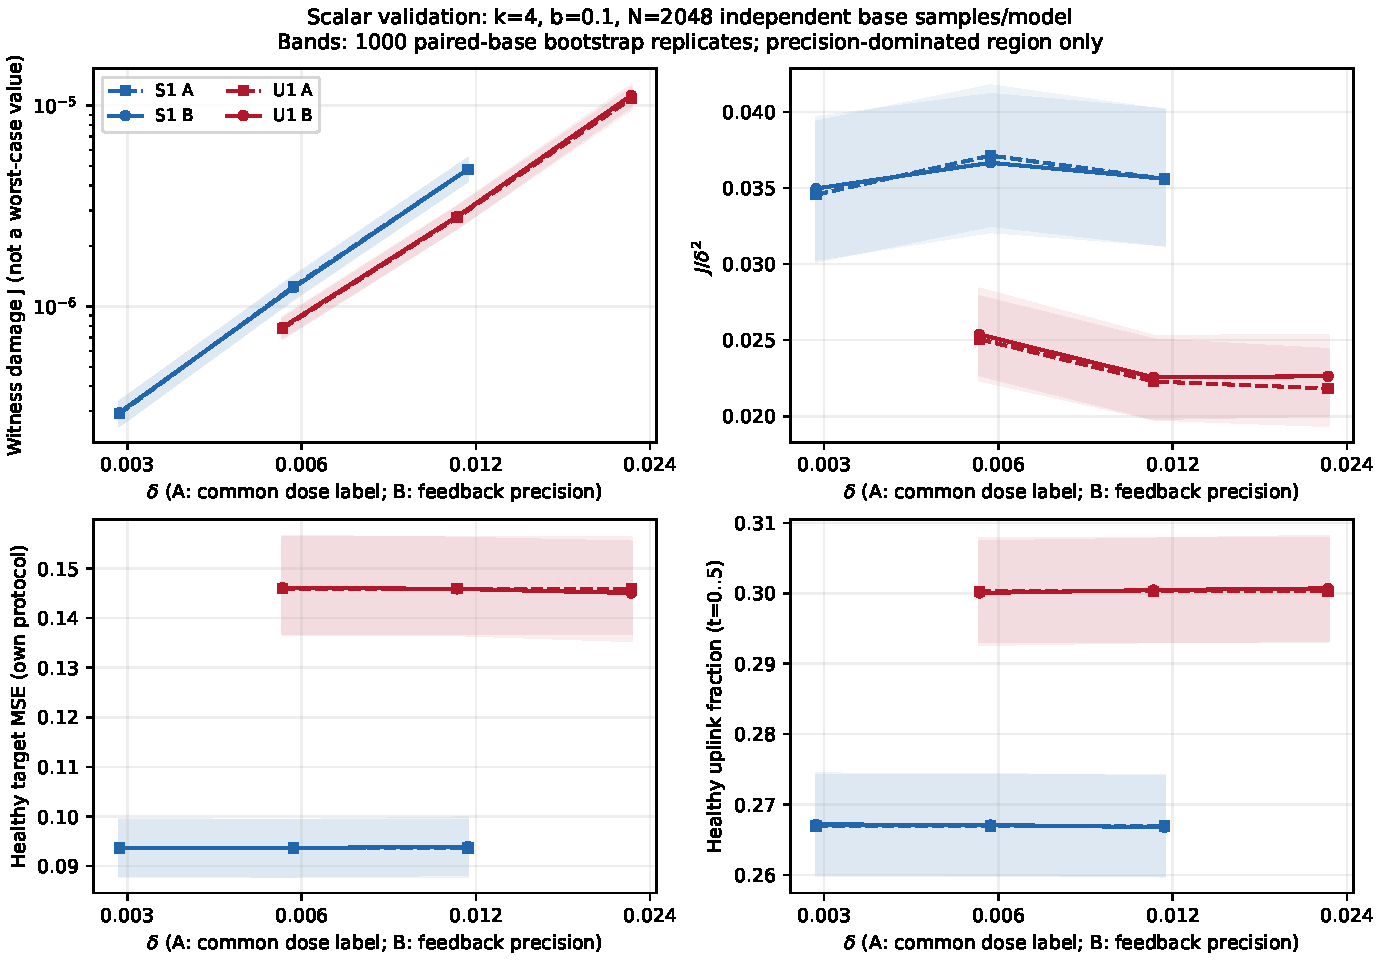
\includegraphics[width=.96\linewidth]{figures/e1_mechanism.pdf}
\end{center}
\noindent
Trusted future events constrain estimation damage under exact prediction feedback.
With scalar quantized feedback, a feasible cell-confined attack preserves the specified telemetry while causing positive damage.
The plots show feasible witnesses, not computed worst-case optima.

\end{document}
